\chapter{Design \& Implementation}\label{sec:impl}

\section{Bitwidth analysis}
The analysis is implemented with the worklist algorithm. The analysis attaches an $(int,boolean)$ tuple to every meaningful node. A node is considered meaningful if the node has an integer-mode. We will reference the first value as \emph{stable bits} and the second value as \emph{is positive}. \newline
What stable here means can be observed when looking at \ref{fig:numbers}.
For the first line of the table we have five stable digits. The second line has 7 stable digits.\newline
With the assumption that both numbers are defined as a signed int. The tuples would be $(4,true)$ and $(6,false)$ for the two numbers from the table.\newline
The whole algorithm is iterative, which means, we might want to address the current tuple $x$ of a node, while we have a new one calculated. Therefore we call $\hat{x}$ the currently associated value, and $x$ the newly calculated one.

\paragraph{Bit representation}
The stable bits indicate how many bits are not used.
The second value of the tuple indicates if the value will ever reach negative numbers or not, it is only meaningful for modes that allow signs. We note down the stable bits of a node as $stable\_nodes(n)$, same for $is\_positive(n)$.
Sometimes we don't want to have the used bits instead of the stable bits, in this case we note the result as: $used\_bits(n):=mode\_bits(n)-stable\_bits(n)$
Where $mode\_bits$ expresses the amount of bits per node.

\paragraph{Range representation}
There is also a second way of interpreting the two values. The stable bits can define a minimum and maximum range. The maximum number is reached if the stable bits are all zero, and the rest one. If the mode is signed and the node is not positive, then the minimum number is reached by assuming all stable bits are one, and the rest zero. Otherwise the minimum is 0. We can define the following min max definitions for the ranges:

$
max_{bitwidth}(n)=
\left\{
\begin{array}{l}2^{used\_bits(n)-1}-1\\2^{used\_bits(n)}-1\end{array}
\begin{array}{l} {mode.signed} \\ {Otherwise} \end{array}
\right.
$

$
min_{bitwidth}(n)=
\left\{
\begin{array}{l}-2^{used\_bits(n)-1}\\0\end{array}
\begin{array}{l} {mode.signed \wedge \neg is\_positive} \\ {Otherwise} \end{array}
\right.
$

\begin{figure}
	\centering
	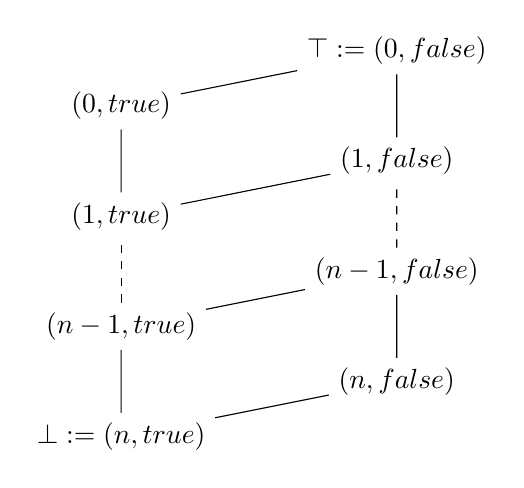
\begin{tikzpicture}[scale=.7]
		\node (np0) at(0,0) {$\bot := (n,true)$};
		\node (np1) at(0,2) {$(n-1,true)$};
		\node (np2) at(0,4) {$(1,true)$};
		\node (np3) at(0,6) {$(0,true)$};
		\node (p0) at(5,1) {$(n,false)$};
		\node (p1) at(5,3) {$(n-1,false)$};
		\node (p2) at(5,5) {$(1,false)$};
		\node (p3) at(5,7) {$\top := (0,false)$};
		\draw (np0) -- (p0) -- (p1) -- (np1) -- (np0);
		\draw (np2) -- (p2) -- (p3) -- (np3) -- (np2);
		\draw [dashed] (np1) -- (np2);
		\draw [dashed] (p1) -- (p2);
	\end{tikzpicture}
\caption{Hesse diagram of the lattice which is used in this analysis}
\label{fig:lattice}
\end{figure}

\paragraph{Analysis}
\label{analysis_explain}
The analysis works as a fixed point iteration, implemented with the work list approach. You can find the used lattive in \autoref{fig:lattice}. The values of the lattice represent the tuples from the analysis.

As a first step, we iterate over every single node and initialize the node with $\bot$ and mark it as \textit{dirty}. If the node is constant, we calculate its bitwidth. Nodes with the opcodes \textit{Const}, \textit{Size} and \textit{Address} are considered constant.

The second step consists of recalculating every \textit{dirty} node in the graph. 
if the stable bits of $x$ are smaller than those from $\hat{x}$, 
then the new value is memorized as $\hat{x}$ of the node. Also every successor of the node is marked as dirty. The used rules for recalculating the nodes are described in \autoref{table_of_rules}.

\subsection{Value prediction}
In addition to the normal analysis results, the fixed point iteration can insert additional confirm nodes. Those confirm nodes help making the analysis more accurate.
First of all we need a few definitions for easier understanding:

\subparagraph{Definition: Upper bounds}
A compare node defines an upper bound if the relation is $<$ and the second operand is constant.\newline
The definition also applies for compare nodes that can be transformed by swapping the two operands and the relation accordingly.

\subparagraph{Definition: Predecessor in a certain block}
In the detection described later, we often need to find a predecessor that is placed in a certain block. Therefore we define:
\begin{center}
$\kappa(a, b) := \{X| X \leftarrow a \wedge X.block = b \}$ 
\end{center}

It will return every node that is located in \textit{b} and is a predecessor of \textit{a}.

\subparagraph{Definition: Constant dependencies}
\begin{figure}
	\centering
	\begin{tikzpicture}
		\node[graph]{
			\begin{tikzpicture}[remember picture]
				\node[block] (startblock) {
					\begin{tikzpicture}


						\node[firm]    (const1) at (3,3) {Const};
						\node[firm]    (const2) at (3,2) {Const};
						\node[firm]    (mul)    at (1,2) {Mul};
						\node[firm]    (add)    at (1,1) {Add};
						\node[firm]    (sub)    at (0,0) {Sub := $\lambda$};
						\node[firm]    (mul2)    at (-0.5,3) {Mul};
						\node[firm]    (mod)    at (1,3) {Mod};

						\draw[dataDependency]    (sub.60)      -- ++(0,0.1) -| (add);
						\draw[dataDependency]    (sub.north)   -- ++(0,0.1) -| (mul2);	
						\draw[dataDependency]    (add.north)     -- ++(0,0.1) -| (mul);
						\draw[dataDependency]    (add.60)      -- ++(0,0.1) -| (const2);
						\draw[dataDependency]    (mul.60)     -- ++(0,0.1) -| (const1);
						\draw[dataDependency]    (mul.north)   -- ++(0,0.1) -| (mod);
						
						\draw[red, thick,dotted]     ($(mul.north west)+(-0.15,0.15)$) rectangle ($(add.south east)+(0.15,-0.15)$);
					\end{tikzpicture}
				};
			\end{tikzpicture}
		};
	\end{tikzpicture}
    %FIXME highlight mul and addli
\caption{A subgraph of a FIRM graph. The result of $\xi(\lambda)$ is highlighted in red}
\label{fig:def:xi}
\end{figure}
While looking at C code we often see that addition and multiplication nodes are used for calculating array addresses or addresses for structure access. Therefore, one operand of the arithmetical operations is often constant. An example for this can be found in \autoref{fig:def:xi}.
We define $\xi$ to explore the whole tree of nodes with one constant and one none-constant operand, and returns every node that was not constant.
\begin{center}
$\xi(a) := 
\left\{
	\begin{array}{l}
		a \cup \xi(c)\\ 
		\emptyset
	\end{array}
	\begin{array}{l}
		, \text{If there is only one not constant dependency \textit{c}} \\ 
		, \text{otherwise}.
	\end{array}
\right.$
\end{center}

If \textit{a} has only one none-constant operand c, then $\xi$ returns the element $a$ and $\xi(c)$. Otherwise it returns an empty set. In \autoref{fig:def:xi} the highlighted nodes are part of $\xi(Y)$.

\paragraph{Upper bounds for block execution}
The values that are calculated in a node are (even if the fixed point iteration is not stable yet) within the ranges for the later stable result. The iteration starts at $\bot$ and moves into the direction of $\top$. 
We now evaluate an upper bound compare node, every time the first operand changes. In the beginning we can say that that with those possible values, each time the true-block will be executed. However, if $max_{bitwidth}(n)$ grows enough to get bigger than the second operand or the compare node, then we can say, that we have found a upper bound for the execution of the true-block. Which is $max _{bitwidth}(n)$ in the current state. Thus we can insert a confirm node between every node $e \in \kappa(i, j)$ and $i$, where $i$ is the first operand and $j$ is the true block.
\label{upper_bound_insert_confirm}

\paragraph{Extended confirm insertion}
The confirm nodes that we have inserted in the paragraph before can also be transported backwards.bot
With $\xi(i)$ we can get a set of nodes, where the current state in the analysis is only depending on one node. Thus we can say that the state of every node from $\xi(i)$ will not change as long as the topmost upper element in the tree structure does not change. Which means that we can insert a confirm node between $(e,g)$ for every $e \in \xi(i)$ and $g \in \kappa(e, j)$. Those additional confirm nodes then must get there bound adjusted, so the confirm nodes do make sense with the arithmetical operation between them.

\section{Stable Conversion nodes}
In $\libFIRM$ a conversion node can be used to convert a value from one mode to another. This type of node has one operand. A conversion like this can have one of two effects. The value stays the same, or the value changes, due to the inability of representing the value in a different mode. We call the first case \textit{stable conversion node}. A example for an unstable conversion node may look like ($unsigned$)(($int$)-10). A stable conversion node may look like ($unsigned$)(($int$)10).

\paragraph{Finding stable conversion nodes}
Such stable conversion nodes can be found using the bitwidth analysis. We compare the range of the operand with the range of the conversion node itself. If the ranges are the same, then we know that the conversion is stable.

\paragraph{Removing conversion nodes}
\begin{figure}
	\centering
	\begin{tikzpicture}[scale=.7]
		\node[graph]{
			\begin{tikzpicture}[remember picture]
				\node[block] (startblock) {
					\begin{tikzpicture}
					
					
					\node[firm]    (conv) at (-1,2) {Conv};
					\node[firm]    (const) at (1,2) {Const};
					\node[firm]    (cmp)    at (0,1) {Cmp};
					\node[firm]    (cond)    at (0,0) {Cond};

					\draw[dataDependency]    (conv.north)   -- ++(0,0) -| (-1,3);	
					
					\draw[dataDependency]    (cmp.60)      -- ++(0,0.1) -| (const);
					\draw[dataDependency]    (cmp.120)      -- ++(0,0.1) -| (conv);
					\draw[dataDependency]    (cond.north)     -- ++(0,0.1) -| (cmp.south);
					
					\end{tikzpicture}
				};
			\end{tikzpicture}
		};
	\end{tikzpicture}
\caption{Conversion compare construction}
\label{fig:example:conversion_opt}
\end{figure}
In case we found a stable conversion node, we can say that this node only exists for syntax rules, there is no semantical value in it. Removing those nodes also has the advantage of helping other analyses. \newline
One example for this is the confirm insertion algorithm of $\libFIRM$, it searches for assertions that can be made based on looking at compare nodes. This works quite well. However, the example in \autoref{fig:example:conversion_opt} does not work. The insertion code can only insert a Confirm between the Compare and the conversion. However, this is not useful for other analysis, therefore the Confirm node should be before the Conv node.
After removing the conversion node, the analysis can find an assertion based on the compare node. Other examples where this can improve things is in the dead code elimination, and the branch prediction. Next two paragraphs are explaining two concrete optimizations for removing conversion nodes.

\paragraph{Compare-Conversion optimization}
The rule in $\libFIRM$ is that two operands of a compare node have to have the same mode. This means, when we remove the conversion node, we also need to adjust the mode of the second operand. This is not easily possible for a none-Constant node.
Thus we confine for now that the operand needs to be a Conversion node, and the second one a Constant node. \newline
With this we can simple adjust its mode, and remove the conversion.

\paragraph{Arithmetical-Conversion optimization}
\begin{figure}
	\centering
	\begin{tikzpicture}[scale=.7]
		\node[inner sep=0pt] (russell) at (0,0){
			\includegraphics[width=.25\textwidth]{fig/arithmetical_opt.png}
		};
	\end{tikzpicture}
\caption{Arithmetical optimization example}
\label{fig:example:arithmetical_opt}
\end{figure}
The situation of arithmetical nodes, with one operation being constant, one being a conversion, can also be optimized. In this case we move it through the arithmetical operation, and place it afterwards. At the same time we change the mode of the constant and the arithmetical node to the not converted mode. We do this in order to hope that we can remove it with a compare conversion optimization after that.
Such a construct might look like \autoref{fig:example:arithmetical_opt} . After we adjusted the mode of the constant we can move the conversion from the operand of the arithmetical operation to the end.

\section{VHDL generation}

There is a $\libFIRM$ tool called firm2vhdl. The tool takes the output from the \textit{cparser} compiler, and outputs the VHDL. Every node in the firm graph gets transformed into a VHDL statement. This is done by transforming the operation of the nodes into VHDL code. Each result of a node operation is assigned to a new variable, which then can be used again later by the next operation. 
Each of those those variables are represented in hardware, and thus have an certain amount of bits. The maximum amount of bits that is needed, can be calculated by using the bitwidth analysis.

\paragraph{bitwidth in firm2vhdl}
The amount of bits per variable were previously just the amount of bits the mode of a node needs. In VHDL this wastes a lot of space on the FPGA chip later on. Minimizing the amount of bits used per variable here can be important, since most of the variables used in C do not use the complete bitwidth.\newline
The bitwidth information gathered from the analysis can help here, as it defines how many bits of a node are used, and how many are not. Thus we can add code to the transformation, for taking the bitwidth, instead of the number of bits in a mode.
\newsavebox{\ccode}
\begin{lrbox}{\ccode}% Store first listing
\begin{lstlisting}
int op(char i, char y) {
	return (int)i + y;
}
\end{lstlisting}
\end{lrbox}

\newsavebox{\opt}
\begin{lrbox}{\opt}% Store first listing
	\begin{tabular}{ l c c }
		node & unoptimized & optimized \\ 
		\hline
		node230 & 8 & 3  \\
		node231 & 32 & 6  \\
		node228 & 8 & 9 \\
		node229 & 32 & 9 \\
		node232 & 32 & 9 \\
	\end{tabular}
\end{lrbox}


\begin{figure}
	\centering
	\hfill
	\subfloat[Sample c code]{\label{fig:firm2vhdl-sample}\usebox{\ccode}}
	\hfill
	\subfloat[VHDL defined variable sizes]{\label{fig:firm2vhdl-table}\usebox{\opt}}
	\hfill
\label{fig:vrp_loop_examples}
\caption{firm2vhdl example}
\end{figure}

As an example, the C code from \ref{fig:firm2vhdl-sample} can be compiled with the tool. Without the optimization the 5 created nodes will have the bit numbers from the first column in \ref{fig:firm2vhdl-table}. However, after we applied out bitwidth analysis, we have the bit usages from the last column in \ref{fig:firm2vhdl-table}. 

\section{Value range vs. bitwidth}

The analysis explained in \ref{analysis_explain} is using rules which are based on the bitwidth. The same algorithm could use rules that are working on the range, and not the bitwidth. The later is called value range propagation. The result of both analyses are similar. However, a master thesis from MIT (\cite{bitwidthanalysis-mit-vrp}) claims that the value range propagation is more accurate than the bitwidth analysis, and not only because of the rounding up.

\begin{figure}
	\centering

	\hfill
	\subfloat[Loop configuration where no assertion is possible]{\label{fig:loop_no_assertions}
	\begin{tikzpicture}
		\node[graph]{
			\begin{tikzpicture}[remember picture]
				\node[block] (startblock) {
					\begin{tikzpicture}
						\node[firm]    (const0) at (0,2) {Const : 0};
						\node[phi]     (phi)    at (-1,1) {Phi};
						\node[firm]    (const1) at (1,1) {Const : 1};
						\node[firm]    (add)    at (0,0) {Add};
						
						\draw[dataDependency]    (add.60)     -- ++(0,0.1) -| (const1);
						\draw[dataDependency]    (add.120)    -- ++(0,0.1) -| (phi);
						\draw[dataDependency]    (phi.60)     -- ++(0,0.1) -| (const0);
						\draw[dataDependency]    (phi.120)    -- ++(0,0.1) -- ++(-1,0) -- ++(0,-2) -| (add);
					\end{tikzpicture}
				};
			\end{tikzpicture}
		};
	\end{tikzpicture}
	}
	\hfill
	\subfloat[Loop configuration where a assertion is possible]{\label{fig:loop_assertions}
	\begin{tikzpicture}
		\node[graph]{
			\begin{tikzpicture}[remember picture]
				\node[block] (startblock) {
					\begin{tikzpicture}
					\node[firm]    (const0) at (0,2) {Const : 0};
					\node[phi]     (phi)    at (-1,1) {Phi};
					\node[firm]    (const1) at (1,1) {Const : 1};
					\node[firm]    (add)    at (0,0) {Add};
					\node[firm]    (cmp)        at ( 0,-1) {Cmp less\_equal};
					\node[control] (cond)       at ( 0,-2) {Cond};
					\node[control] (false)      at (-1,-3) {False};
					\node[control] (true)       at ( 1,-3) {True};
					
					\draw[dataDependency]    (add.60)      -- ++(0,0.1) -| (const1);
					\draw[dataDependency]    (add.120)     -- ++(0,0.1) -| (phi);
					\draw[dataDependency]    (phi.60)      -- ++(0,0.1) -| (const0);
					\draw[dataDependency]    (phi.120)     -- ++(0,0.1) -- ++(-1,0) -- ++(0,-2) -| (add.240);
					\draw[dataDependency]    (cmp.62)     --              (add.300);
					\draw[dataDependency]    (cond)        --              (cmp);
					\draw[controlDependency] (false.north) -- ++(0,0.1) -| (cond.240);
					\draw[controlDependency] (true.north)  -- ++(0,0.1) -| (cond.300);
					
					\end{tikzpicture}
				};
			\end{tikzpicture}
		};
	\end{tikzpicture}
	}
	\hfill
	\caption{Possible loop configurations}
\label{fig:vrp_loop_examples}
\end{figure}


However, the thesis misses one essential fact. In case of a loop like \autoref{fig:loop_no_assertions}, where no assertions can be made, both analyses share the same result: The nodes will use their whole bitwidth / range. However, the difference between the two analysis here is, that the VRP will need $2^{msb}$ iterations, while the bitwidth analysis only takes $msb$ iterations, where $msb$ expresses the number of the maximum bit. Thus the bitwidth analysis produces the same result, while it's a lot faster.

Another interesting situation is when a Confirm node can be inserted in a loop (See \ref{fig:loop_assertions}). If this is the case, then the bitwidth analysis will return $2^{\lceil log2(bound) \rceil}$ while the VRP would return $log2(bound)$ as the biggest number required by the code. What this shows is, that the VRP here is only more accurate, because the data structure of the bitwidth info operates on bits, while the VRP operates on normal numbers. The runtime here is the same.

\begin{figure}
	\centering
	\begin{tikzpicture}
		\node[graph]{
			\begin{tikzpicture}[remember picture]
				\node[block] (startblock) {
					\begin{tikzpicture}
					\node[firm]    (add1)    at (-2,2) {Add};
					\node[firm]    (add2)    at (0,2) {Add};
					\node[firm]    (mul)    at (-1,1) {Mul};
					\node[firm]    (const3) at (1,1) {Const};
					\node[firm]    (sub)    at (0,0) {Sub};
					
					\draw[dataDependency]    (mul.60)      -- ++(0,0.1) -| (add2);
					\draw[dataDependency]    (mul.120)      -- ++(0,0.1) -| (add1);
					\draw[dataDependency]    (sub.60)      -- ++(0,0.1) -| (const3);
					\draw[dataDependency]    (sub.120)      -- ++(0,0.1) -| (mul);
					
					\end{tikzpicture}
				};
			\end{tikzpicture}
		};
	\end{tikzpicture}
	\caption{Possible loop configurations}
\label{fig:arithmetical_chains}
\end{figure}
\label{VRP_king}
The only configuration where the VRP returns constantly a more accurate result, is when arithmetical operations are not looping, but are rather used as some sort of tree structure, like it is illustrated in \ref{fig:arithmetical_chains}. Here the VRP is more accurate, the runtime is the same. However, this drawback can be fixed, and will be covered in a later section.

